\documentclass[10pt,aspectratio=169,english,fontset=none]{beamer}
% \overfullrule=1pt
\usepackage[fontset=none]{ctex}
\usepackage{hologo}
\usepackage{luamesh}
\usepackage{mtpro2}
\usepackage{babel}
\usepackage{pgfpages}
\usepackage{cncolours}
\definecolor{nuanbai}{HTML}{f5f5f5} % F5F5F5
\usepackage[most]{tcolorbox}
\usepackage{biblatex}
\hypersetup{colorlinks=true,linkcolor=red,citecolor=red}
\usetikzlibrary{shadows}
\usetikzlibrary{calc}
\tcbuselibrary{listings,breakable}
\tcbuselibrary{documentation}
\tcbset{
    color command=AmurmapleRed,
    color environment=AmurmapleRed,
    color option=AmurmapleGreen
}
\definecolor{bg}{HTML}{e0e0e0}
\definecolor{fg}{HTML}{455a64}

\usetheme[
%nogauge,
sidebar,sidebarwidth=58pt,
nomail,
delaunay,
amurmapleblue
]{Amurmaple}
\setbeamertemplate{background}{
\includegraphics[width=\paperwidth,height=\paperheight]{figures/bg.pdf}}
%bg-image 是背景图片名称,亲测png和pdf和jpg可行,eps不行
\lstset{
  numberstyle=\footnotesize\color{gray},
  keywordstyle=\ttfamily\bfseries\color{structure},
  basicstyle=\ttfamily\normalsize,
  commentstyle=\itshape\color{gray},
  stringstyle=\ttfamily,
  showstringspaces=false,
  language=[LaTeX]TeX,
  breaklines=true,
  breakindent=30pt,
  defaultdialect=[LaTeX]TeX,
  morekeywords={usetheme,definecolor, beamerbutton, beamerskipbutton,
    beamerreturnbutton, structure, alert, sectionpage, mail, webpage,
    collaboration, subtitle, institute, titlegraphic, sepframe, includegraphics,
    thanksframe, inserttitlegraphic, framesection, boxalert,appendix}
  % frame=tb
}
\pgfdeclarelayer{background} %背景%底层
\pgfdeclarelayer{foreground} %上层
\pgfdeclarelayer{top} %顶部
\pgfdeclarelayer{bottom} %底部
\pgfsetlayers{bottom,background,main,foreground,top}

\makeatletter
% 第一种定理
\tcbset{my@basic@thm/.style={enhanced jigsaw, breakable, 
  enlarge left by=-3.5mm, width=\textwidth+3.5mm, boxrule=0pt, 
  top=2pt, bottom=2pt, left=2.5mm, frame hidden}}
\newcommand{\@my@newtheorem@n}[1]{\ERROR}
\newcommand{\@my@newtheorem@nn}[2]{%
  \@ifundefined{#1}{\@my@newtheorem{#1}#2}{\@my@renewtheorem{#1}#2}}
\NewDocumentCommand{\@my@newtheorem}{ m m o +m }
  {\IfNoValueTF{#3}{\newtheorem{#1}{#2}}{\newtheorem{#1}{#2}[#3]}%
    \tcbset{my@#1@thmstyle/.style={#4}}%
    \tcolorboxenvironment{#1}{my@basic@thm, my@#1@thmstyle}}
\NewDocumentCommand{\@my@renewtheorem}{ m m o +m }
  {\IfNoValueTF{#3}{\renewtheorem{#1}{#2}}{\renewtheorem{#1}{#2}[#3]}%
    \tcbset{my@#1@thmstyle/.style={#4}}}
%
% ---------------------------------------------------------------------------------- %
% 第二种定理
\tcbset{my@basic@tcbthm/.style={detach title,}}
\newcommand{\@my@newtcbtheorem@n}[1]{\ERROR}
\newcommand{\@my@newtcbtheorem@nn}[2]{%
  \@ifundefined{#1}{\@my@newtcbtheorem{#1}{#2}}{\@my@renewtcbtheorem{#1}{#2}}}
\newcommand{\@my@newtcbtheorem}[2]{%
  \edef\my@curr@thmenvname{#1}% 它保存当前定理环境的名称
  \mytcbtheoremset{#2}%
  \NewTColorBox{#1}{ O{} O{} o }
    {my@basic@tcbthm, my@#1@tcbthmstyle, title={##2}, IfNoValueF={##3}{label={##3}}, ##1}}
\newcommand{\@my@renewtcbtheorem}[2]{\edef\my@curr@thmenvname{#1}\mytcbtheoremset{#2}}

% 键值设置
\pgfkeys{/mytcbtheorem/.is family}
\newcommand{\mytcbtheoremset}{\pgfqkeys{/mytcbtheorem}}
\mytcbtheoremset{
  name/.code=\@namedef{\my@curr@thmenvname @name}{#1}, %无效
  counter/.code=\@namedef{my@\my@curr@thmenvname @counter}{#1}\newcounter{#1},
  the counter/.code=\@namedef{the\@nameuse{my@\my@curr@thmenvname @counter}}{#1},
  autoref name/.code=\@namedef{\@nameuse{my@\my@curr@thmenvname @counter}autorefname}{#1},
  style/.code=\tcbset{my@\my@curr@thmenvname @tcbthmstyle/.style={#1}},
  thmcolor/.code=\@namedef{\my@curr@thmenvname @thmcolor}{#1}, %无效
  lemcolor/.code=\@namedef{\my@curr@thmenvname @lemcolor}{#1}, %无效
}
% 存储键值 (LaTeX3)
\ExplSyntaxOn
\cs_new_protected:Npn \mynewtheorem 
  { \keyval_parse:NNn \@my@newtheorem@n \@my@newtheorem@nn }
\cs_new_protected:Npn \mynewtcbtheorem
  { \keyval_parse:NNn \@my@newtcbtheorem@n \@my@newtcbtheorem@nn }
\ExplSyntaxOff
\makeatother

% 第二种定理
\makeatletter
%%  Overlay Settings
\newcommand{\my@theorem@overlay@unbroken}[2]{
  \def\trianglelen{0.75cm}
      %%============== First ==============%% 
  \fill[black!60] ([xshift=\trianglelen,yshift=5pt]frame.north west)-- ([xshift=\trianglelen-0.2cm,yshift=0cm]frame.north west)--([xshift=0.2cm+\trianglelen,yshift=0cm]frame.north west)--cycle;
  \node[rectangle, text=white, drop shadow={opacity=.3, shadow xshift=0.1cm}, inner sep=1mm,fill=#2,
anchor=west,rounded corners=3pt,font=\bfseries\normalsize] at ([xshift=0cm,yshift=-2mm]frame.north west) {\hspace*{1.6em}#1.~\tcbtitletext};
  \fill[color=#2,drop shadow={opacity=0.3,shadow xshift=.3pt}] 
      ([xshift=\trianglelen,yshift=5pt]frame.north west) {[rounded corners=3pt]--++(-\trianglelen-5pt,0)}--++(0,-\trianglelen-5pt)--cycle;
  \fill[color=black!60] ([xshift=-5pt,yshift=-\trianglelen]frame.north west)--([xshift=0cm,yshift=-\trianglelen+0.2cm]frame.north west)-- ([xshift=0cm,yshift=-0.2cm-\trianglelen]frame.north west)--cycle;
      %%============== End ==============%% 
  \fill[#2,drop shadow={opacity=0.3,shadow xshift=-0.008\linewidth,shadow yshift=0.0016\linewidth}] 
  ([xshift=-0.05\linewidth,yshift=-5pt]frame.south east) {[rounded corners=3pt]--++(0.05\linewidth+5pt,0)}--++(0,0.05\linewidth+5pt)--cycle;
  \fill[black!60] ([xshift=-0.05\linewidth,yshift=-5pt]frame.south east) -- ([xshift=-0.04\linewidth,yshift=0pt]frame.south east)-- ([xshift=-0.06\linewidth,yshift=0pt]frame.south east)--cycle;
  \fill[black!60] ([xshift=5pt,yshift=0.05\linewidth]frame.south east)-- ([yshift=0.04\linewidth]frame.south east) -- ([yshift=0.06\linewidth]frame.south east)--cycle;
}
\newcommand{\my@theorem@overlay@first}[2]{
  \def\trianglelen{0.75cm}
  \fill[black!60] ([xshift=\trianglelen,yshift=5pt]frame.north west)-- ([xshift=\trianglelen-0.2cm,yshift=0cm]frame.north west)--([xshift=0.2cm+\trianglelen,yshift=0cm]frame.north west)--cycle;
  \node[rectangle, text=white, drop shadow={opacity=.3, shadow xshift=0.1cm}, inner sep=1.5mm,fill=#2, anchor=west,rounded corners=3pt,font=\bfseries\normalsize] at ([xshift=0cm,yshift=-2mm]frame.north west) {\hspace*{1.6em}#1.~\tcbtitletext};
  \fill[color=#2,drop shadow={opacity=0.3,shadow xshift=.3pt}] 
        ([xshift=\trianglelen,yshift=5pt]frame.north west) {[rounded corners=3pt]--++(-\trianglelen-5pt,0)}--++(0,-\trianglelen-5pt)--cycle;
  \fill[color=black!60] ([xshift=-5pt,yshift=-\trianglelen]frame.north west)--([xshift=0cm,yshift=-\trianglelen+0.2cm]frame.north west)-- ([xshift=0cm,yshift=-0.2cm-\trianglelen]frame.north west)--cycle;
}
\newcommand{\my@theorem@overlay@last}[1]{
  \fill[#1,drop shadow={opacity=0.3,shadow xshift=-0.008\linewidth,shadow yshift=0.0016\linewidth}] 
  ([xshift=-0.05\linewidth,yshift=-5pt]frame.south east) {[rounded corners=3pt]--++(0.05\linewidth+5pt,0)}--++(0,0.05\linewidth+5pt)--cycle;
  \fill[black!60] ([xshift=-0.05\linewidth,yshift=-5pt]frame.south east) -- ([xshift=-0.04\linewidth,yshift=0pt]frame.south east)-- ([xshift=-0.06\linewidth,yshift=0pt]frame.south east)--cycle;
  \fill[black!60] ([xshift=5pt,yshift=0.05\linewidth]frame.south east)-- ([yshift=0.04\linewidth]frame.south east) -- ([yshift=0.06\linewidth]frame.south east)--cycle;
}
% Second theorem style overlay settings 
\newcommand{\my@lemma@overlay@unbroken}[2]{
    %%============== First ==============%%
    \def\Rad{3.5pt}
    \def\theight{0.45cm}
    \def\rad{7pt}%
    \path[fill=#2,drop shadow={opacity=0.3,shadow xshift=.05cm,shadow yshift=-.05cm}]node[append after command={
    ([xshift=-1.5*\rad]thmname.north west) to[out=0,in=180,looseness=1] ([xshift=2.5*\rad]thmname.south west) --([xshift=-\rad]thmname.south east) to[out=0,in=180,looseness=1] ([xshift=3*\rad]thmname.north east) --cycle},
    text=white,font=\bfseries,align=center,inner ysep=1.5mm,right] (thmname) at ([xshift=\rad,yshift=-\rad]frame.north west) {\hspace*{10pt}#1. \tcbtitletext};
    \begin{pgfonlayer}{bottom}
      \fill[#2,opacity=0.5]
      ([xshift=-1.5*\rad]thmname.north west) to[out=-90,in=0,looseness=1.5] +(3pt,-6pt) -| +(10pt,0)--cycle;
      \fill[#2,opacity=0.5]
      ([xshift=3*\rad]thmname.north east) to[out=0,in=-90] +(5pt,-5pt) -| ++(-10pt,0) --cycle;
    \end{pgfonlayer}
    %%============== End ==============%%  
    \def\tlen{1.5cm}
    \path[fill=#2,drop shadow={opacity=0.3,shadow xshift=.3pt}]
    ([xshift=-2*\rad,yshift=-5pt]frame.south east) coordinate (SE)  to[out=0,in=180] +(4*\rad,5pt+\theight) --([shift={(-\tlen+4*\rad,5pt+\theight)}]SE) to[out=180,in=0] +(-4*\rad,-5pt-\theight) --cycle;
    \begin{pgfonlayer}{bottom}
      \fill[color=#2!80!black] ([xshift=-1.35*\tlen+\Rad,yshift=-5pt]frame.south east) to[out=180,in=90,looseness=0.7] ([xshift=-1.35*\tlen-0.5*\Rad]frame.south east) coordinate (NWl)--([xshift=2*\rad]NWl) to[out=-90,in=-180,looseness=0.7] ([xshift=-1.35*\tlen+\Rad,yshift=-5pt]frame.south east)--cycle;
    \end{pgfonlayer}
	}
\newcommand{\my@lemma@overlay@first}[2]{
    %%============== First ==============%%
    \def\Rad{3.5pt}
    \def\theight{0.57cm}
    \def\rad{7pt}%
    \path[fill=#2,drop shadow={opacity=0.3,shadow xshift=.05cm,shadow yshift=-.05cm}]node[append after command={
    ([xshift=\rad]thmname.north west) to[out=180,in=0,looseness=1] ([xshift=-3*\rad]thmname.south west) --([xshift=-\rad]thmname.south east) to[out=0,in=180,looseness=1] ([xshift=3*\rad]thmname.north east) --cycle},
    text=white,font=\bfseries,align=center,inner ysep=1.5mm,right] (thmname) at ([xshift=\rad,yshift=-\rad]frame.north west) {\hspace*{10pt}#1.\ \tcbtitletext};
  }
\newcommand{\my@lemma@overlay@last}[1]{
    %%============== End ==============%%  
    \def\Rad{3.5pt}
    \def\rad{7pt}%
    \def\theight{0.45cm}
    \def\tlen{1.5cm}
    \path[fill=#1,drop shadow={opacity=0.3,shadow xshift=.3pt}]
    ([xshift=-2*\rad,yshift=-5pt]frame.south east) coordinate (SE)  to[out=0,in=180] +(4*\rad,5pt+\theight) --([shift={(-\tlen+4*\rad,5pt+\theight)}]SE) to[out=180,in=0] +(-4*\rad,-5pt-\theight) --cycle;
    \begin{pgfonlayer}{bottom}
      \fill[color=#1!80!black] ([xshift=-1.35*\tlen+\Rad,yshift=-5pt]frame.south east) to[out=180,in=90,looseness=0.7] ([xshift=-1.35*\tlen-0.5*\Rad]frame.south east) coordinate (NWl)--([xshift=2*\rad]NWl) to[out=-90,in=-180,looseness=0.7] ([xshift=-1.35*\tlen+\Rad,yshift=-5pt]frame.south east)--cycle;
    \end{pgfonlayer}
	}
\makeatother
%%  
%% 定义第一种定理
\definecolor{CyaN}{HTML}{dbe1e5}
\colorlet{OrangE}{yellow!20!orange}
\colorlet{BluE}{cyan!70!blue}
\colorlet{ReD}{red!20!orange}
\colorlet{GreeN}{yellow!40!green}
\mynewtheorem{
    Defi={\textbf{Definition}}[section]{colback=CyaN!80, borderline west={1.5mm}{0mm}{ReD}},
    Thm={\textbf{Theorem}}[section]{colback=CyaN, borderline west={1.5mm}{0mm}{CyaN!80!black}},
    Lem={\textbf{Lemma}}[section]{colback=CyaN!80, borderline west={1.5mm}{0mm}{BluE}},
    Prop={\textbf{Proposition}}[section]{colback=CyaN!80, borderline west={1.5mm}{0mm}{OrangE}},
    Exam={\textbf{Example}}[section]{colback=CyaN!80, borderline west={1.5mm}{0mm}{DarkGreen}},
    Cor={\textbf{Corollary}}[section]{colback=CyaN!80, borderline west={1.5mm}{0mm}{violet}},
}
%\newtheorem*{remark}{\textbf{Remark}}
%% 定义第二种定理
%%  用法
% % theorem 环境
% overlay unbroken=\my@theorem@overlay@unbroken{\theorem@name\ \thetcbthm}{额外的选项}
% overlay first=\my@theorem@overlay@first{\theorem@name\ \thetcbthm}{额外的选项}
% % lemma 环境
% overlay unbroken=\my@theorem@overlay@unbroken{\lemma@name\ \thetcblemma}{额外的选项}
%% 用户接口区
\usepackage{ninecolors}
\definecolor{examback}{HTML}{e3e6e8}
\makeatletter
\mynewtcbtheorem{
    % 这个 theorem 是环境名
    thm={
        counter=tcbthm, 
        the counter=\thesection.\arabic{tcbthm}, 
%        name=Theorem, % 它保存到 \theorem@name 里
%        thmcolor=purple5,
        autoref name=\bfseries Theorem, 
        style={
        arc=3pt,breakable,enhanced,interior style={top color=AmurmapleBlue!5 ,middle color=AmurmapleBlue!1!nuanbai, bottom color=nuanbai},boxrule=0pt,top=6mm,
        fuzzy shadow={-0.6mm}{0.6mm}{0mm}{0.3mm}{white!50!gray},% 上
        fuzzy shadow={0.6mm}{-0.6mm}{0mm}{0.3mm}{fill=white!40!gray},%下
        opacityframe=0, opacityback=0.98,
        fontupper=\itshape, step={tcbthm},
        before pre=\smallskip, after app=\smallskip,
        overlay unbroken=\my@theorem@overlay@unbroken{定理\ \thetcbthm}{AmurmapleBlue},
        overlay first=\my@theorem@overlay@first{定理\ \thetcbthm}{AmurmapleBlue},
        overlay last=\my@theorem@overlay@last,
        }
    },
    prop={
        counter=tcbprop, 
        the counter=\thesection.\arabic{tcbprop}, 
        autoref name=\bfseries Proposition, 
        style={
        arc=3pt,breakable,enhanced,colback=nuanbai,boxrule=0pt,top=6mm,
        fuzzy shadow={-0.6mm}{0.6mm}{0mm}{0.3mm}{white!50!gray},% 上
        fuzzy shadow={0.6mm}{-0.6mm}{0mm}{0.3mm}{fill=white!40!gray},%下
        opacityframe=0, opacityback=0.98,
        fontupper=\itshape, step={tcbprop},
        before pre=\smallskip, after app=\smallskip,
        overlay unbroken=\my@theorem@overlay@unbroken{Proposition\ \thetcbprop}{DeepPink},
        overlay first=\my@theorem@overlay@first{Proposition\ \thetcbprop}{DeepPink},
        overlay last=\my@theorem@overlay@last{DeepPink},
        }
    },
    defi={
        counter=tcbdefi, 
        the counter=\thesection.\arabic{tcbdefi}, 
        autoref name=\bfseries Definition, 
        style={
        arc=3pt,breakable,enhanced,colback=nuanbai,boxrule=0pt,top=6mm,
        fuzzy shadow={-0.6mm}{0.6mm}{0mm}{0.3mm}{white!50!gray},% 上
        fuzzy shadow={0.6mm}{-0.6mm}{0mm}{0.3mm}{fill=white!40!gray},%下
        opacityframe=0, opacityback=0.98,
        fontupper=\itshape, step={tcbdefi},
        before pre=\smallskip, after app=\smallskip,
        overlay unbroken=\my@theorem@overlay@unbroken{Definition\ \thetcbdefi}{紫棠},
        overlay first=\my@theorem@overlay@first{Definition\ \thetcbdefi}{紫棠},
        overlay last=\my@theorem@overlay@last{紫棠},
        }
    },
    lem={
        counter=tcblem,
        the counter=\thesection.\arabic{tcblem},
        %name=Lemma, 
        %lemcolor=靛蓝, 
        autoref name=\bfseries Lemma,
        style={
        arc=0mm,breakable,enhanced,interior style={top color=靛蓝!5 ,middle color=靛蓝!1!nuanbai, bottom color=nuanbai},arc=3pt,boxrule=0pt,top=5mm,bottom=5mm,
        fuzzy shadow={-0.6mm}{0.6mm}{0mm}{0.3mm}{white!50!gray},% 上
        fuzzy shadow={0.6mm}{-0.6mm}{0mm}{0.3mm}{fill=white!40!gray},%下
        opacityframe=0, opacityback=0.98,
        fontupper=\normalsize,step={tcblem},
        before pre=\smallskip, after app=\smallskip,
        overlay unbroken=\my@lemma@overlay@unbroken{引理\ \thetcblem}{靛蓝},
        overlay first=\my@lemma@overlay@first{引理\ \thetcblem}{靛蓝},
        overlay last=\my@lemma@overlay@last{靛蓝},
        }
    },
    cor={
        counter=tcbcor,
        the counter=\thesection.\arabic{tcbcor},
        autoref name=\bfseries Corollary,
        style={
        arc=0mm,breakable,enhanced,colback=茶色!1!nuanbai,arc=3pt,boxrule=0pt,top=5mm,bottom=5mm,
        fuzzy shadow={-0.6mm}{0.6mm}{0mm}{0.3mm}{white!50!gray},% 上
        fuzzy shadow={0.6mm}{-0.6mm}{0mm}{0.3mm}{fill=white!40!gray},%下
        opacityframe=0, opacityback=0.98,
        fontupper=\normalsize,step={tcbcor},
        before pre=\smallskip, after app=\smallskip,
        overlay unbroken=\my@lemma@overlay@unbroken{Corollary\ \thetcbcor}{茶色},
        overlay first=\my@lemma@overlay@first{Corollary\ \thetcbcor}{茶色},
        overlay last=\my@lemma@overlay@last{茶色},
        }
    },
    exam={
        counter=tcbexam,
        the counter=\thesection.\arabic{tcbexam},
        autoref name=\bfseries Example,
        style={
        arc=0mm,breakable,enhanced,colback=examback,arc=3pt,boxrule=0pt,top=5mm,bottom=5mm,
        fuzzy shadow={-0.6mm}{0.6mm}{0mm}{0.3mm}{white!50!gray},% 上
        fuzzy shadow={0.6mm}{-0.6mm}{0mm}{0.3mm}{fill=white!40!gray},%下
        opacityframe=0, opacityback=0.98,
        fontupper=\normalsize,step={tcbexam},
        before pre=\smallskip, after app=\smallskip,
        overlay unbroken=\my@lemma@overlay@unbroken{Example\ \thetcbexam}{黛绿},
        overlay first=\my@lemma@overlay@first{Example\ \thetcbexam}{黛绿},
        overlay last=\my@lemma@overlay@last{黛绿},
        }
    },
}
\makeatother
\newenvironment{Note}[1][\bf Note:]{\par\Line\uuline{#1} }{\par\Line}
\newcommand{\Line}{\noindent\tikz\draw[line width=0.65pt,gray!80,dashed] (0,0)--++(.99\linewidth,0);\par}
\newcommand{\Wedge}[1][]{\tikz\path [draw,line width=1pt] (0,0)--++(4pt,12pt) node[right,font=\scriptsize] {#1} --++(4pt,-12pt);}

\newtcblisting{Code}{%
  arc=0pt,outer arc=0pt,
  colback=structure!3,
  colframe=structure,
  breakable,
  boxsep=0pt,left=5pt,right=5pt,top=5pt,bottom=5pt, bottomtitle =
  3pt, toptitle=3pt,
  boxrule=0pt,bottomrule=0.5pt,toprule=0.5pt, toprule at break =
  0pt, bottomrule at break = 0pt,
  listing options={breaklines,basicstyle=\ttfamily},listing only,
}

\newtcblisting{Exemple}{%
  arc=0pt,outer arc=0pt,
  colback=structure!3,
  colframe=structure,
  breakable,
  boxsep=0pt,left=3pt,right=3pt,top=2pt,bottom=2pt, bottomtitle =
  0pt, toptitle=0pt,
  boxrule=0pt,bottomrule=0.5pt,toprule=0.5pt, toprule at break =
  0pt, bottomrule at break = 0pt,
  listing options={breaklines,basicstyle=\ttfamily},
}

\newtcblisting{CodePreambule}{%
  arc=0pt,outer arc=0pt,
  colback=AmurmapleBlue!5,
  colframe=AmurmapleBlue,
  breakable,
  boxsep=0pt,left=5pt,right=5pt,top=5pt,bottom=5pt, bottomtitle =
  3pt, toptitle=3pt,
  boxrule=0pt,bottomrule=0.5pt,toprule=0.5pt, toprule at break =
  0pt, bottomrule at break = 0pt,
  enhanced,
  overlay  ={%
    \node[ minimum width=1cm,
      anchor=south east,yshift=-0cm,fill=AmurmapleBlue] at (frame.south east)
      {\itshape\color{white} preamble};
      % \node[ minimum width=1cm,
      % anchor=south east,yshift=-0cm,color=gray,opacity=0.7] at (frame.south east)
      % {\itshape\small préambule};
  },
  listing options={
    breaklines,
    basicstyle=\ttfamily,
  },listing only,
}
% 浮动环境设置
% 默认情况下, \LaTeX{} 要求每页的文字至少占据 20%,否则该页就只单独放置一个浮动环境,
% 而这通常不是我们想要的, 我们将这个要求降低到 5%.
 \renewcommand*{\textfraction}{0.05}
% 有时如果多个浮动环境连续放在一起, \LaTeX{}
% 会将它们分在几个不同页,即使它们可在同一页放
% 得下. 我们可以通过修改 |\topfraction| 和 |\bottomfraction| 分别设置顶端和底端的浮
% 动环境的最大比例.
 \renewcommand*{\topfraction}{0.9}
 \renewcommand*{\bottomfraction}{0.8}
% 有时\LaTeX{}会把一个浮动环境单独放在一页,
% 我们要求这个环境至少要占据 85% 才能单独放在一页.
% 注意:  |\floatpagefraction| 的数值必须小于 |\topfraction|.
 \renewcommand*{\floatpagefraction}{0.85}
% 关于图片 graphicx
 % 如果图片没有指定后缀, 依次按下列顺序搜索
\DeclareGraphicsExtensions{.pdf,.eps,.jpg,.png}
 % 设置图表搜索路径, 可以给图表文件夹取如下名字
\graphicspath{{figures/}{figure/}{pictures/}%
  {picture/}{pic/}{pics/}{image/}{images/}}

\title[{``它展现给我们微妙而精细的对应, 仿佛来自虚空"}]{{ 仿佛来自虚空-代数几何“教皇”\\ Alexandre Grothendieck}}
\author[Grothendieck]{陆世龙}
\subtitle{Alexandre Grothendieck的故事}
\institute[GXMU]{22级基础数学 202220701001284}
\date{\today}
\titlegraphic{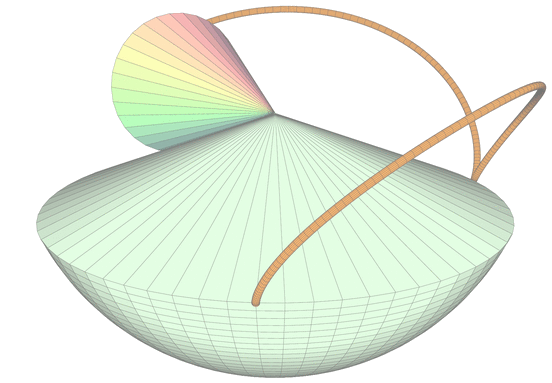
\includegraphics[width=4cm]{logo.png}}
\mail{h1479840692@163.com}
\webpage{https://github.com/BeautyLaTeX/latex-template}
\collaboration{“构成一个研究人员的创造力和想象力的品质的东西,正是他聆听事情内部声音能力”}

\bibliography{ref.bib}
\usefonttheme{serif}
\setmainfont{Fira Sans}
\setsansfont{Times New Roman}
\setCJKmainfont[Path=fonts/]{方正黑体_GBK.TTF}
\setCJKsansfont[Path=fonts/]{方正新书宋_GBK.TTF}
\setCJKmonofont[Path=fonts/]{方正楷体_GBK.TTF}
% \setmathfont{Fira Math}
\usepackage{csquotes}
\setbeamercolor{structure}{bg=black!5}
\usepackage{indentfirst}
% \setmainfont{Times New Roman}
\setlength{\parindent}{2em}

\begin{document}

\maketitle
\sepframe[title={目\quad \quad 录}]

\section{人\ 物\ 简\ 介}
\sepframe[title={人\ 物\ 简\ 介}, image ={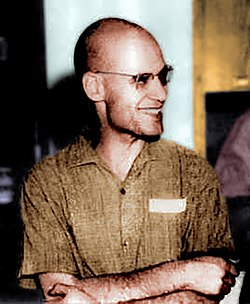
\includegraphics[width =3.4cm]{Alexander_Grothendieck_colorized}}]
\begin{frame}[fragile]{Alexandre Grothendieck的简要介绍}
\begin{abstract}
  亚历山大·格罗滕迪克,1928年3月28日在德国柏林出生 ,犹太裔无国籍数学家.  亚历山大·格罗腾迪克生于德国,1966年获菲尔兹奖,他创立了一整套\boxalert{现代代数几何学}抽象理论体系,对\alert{同调代数}也有建树.
\end{abstract}

\end{frame}

\begin{frame}[fragile]{Alexandre Grothendieck的简要介绍}
    \begin{itemize}[<+-|alert@+>]
\item 1938年,格罗滕迪克10岁时和家人一起作为难民移居法国. 1942年,他的父亲被纳粹杀害,1945年之后,他和母亲被送到集中营,才获得了自由. 之后,格罗滕迪克和他的母亲在蒙彼利埃的一个小村庄定居,他很少去学校,喜欢自学,并且自己研究体积的概念,从中他“发现”测度.

1947年,格罗滕迪克有幸获得法国大学互助协会的奖学金,来到巴黎.这时,他从大学数学教授那里得知,他的测度概念早在1902年就由数学家亨利·勒贝格提出来了. 他很幸运得到了伟大数学家亨利·嘉当的推荐,进入了巴黎高等师范学院的研究班.后来,格罗滕迪克在布尔巴基学派成员洛朗·施瓦茨教授的指导下学习.

格罗滕迪克在读书和研究工作上都十分的努力,后来同学还回忆说,他一直过这没日没夜的孤独生活,每天也都是以香蕉和牛奶度日,完全沉浸在自己的数学迷宫里面.而且格罗滕迪克曾经在选择这所学校的时候,还在数学和音乐上犹豫过,只是因为数学更容易谋生,才这样选择。没想到,如此在数学上有天赋的人,竟然在相差这么大的两个领域中犹豫过.

由于小时候比较困苦的经历,他一直与自己的母亲相依为命,在1957年的时候母亲去世以后,他停止了所有关于数学的研究和学术活动,说要当一个作家,去找寻自我. 不过几个月后,又选择回到了数学。 那是1958年, 也是他数学生涯中最多产的一年.
    \end{itemize}
    \vspace{-\baselineskip}\hfill\beamerskipbutton{Skip Button}
\end{frame}

\begin{frame}[fragile]{续接上文}
  在这一年里,一个著名的法国高等科学研究院被成立了,而他就是其中的创始成员之一.而且在这个研究所里面是没有什么书籍的,格罗滕迪克解释道他们不读书, 只写书. 在这里的一段时间, 他开辟了自己的几何亡国, 被称为代数几何“圣经”的《代数几何原理》的前8卷就是在1960 $\sim $ 1967年间他与让• 迪厄多内在这里一起合作完成的.

他被后来的代数几何学家冠以“教主”的称号。这个研究院是世界上最重要的的代数几何学研究中心,其实很大的程度上就是因为格罗滕迪克和他的工作.

\begin{quotation}[---------《收获与播种》,第 20 页]
  每一门科学,当我们不是将它作为能力和统治力的工具,而是作为我们人类世代以来孜孜以求的对知识的冒险历程,不是别的,就是这样一种和谐, 从一个时期到另一个时期,或多或少,巨大而又丰富.  在不同的时代和世纪中,对于依次出现的不同的主题,它展现给我们微妙而精细的对应,仿佛来自虚空.
\end{quotation}
\end{frame}

\section{Alexandre Grothendieck的部分工作概述}
\sepframe[title={Alexandre Grothendieck的部分工作概述}, image ={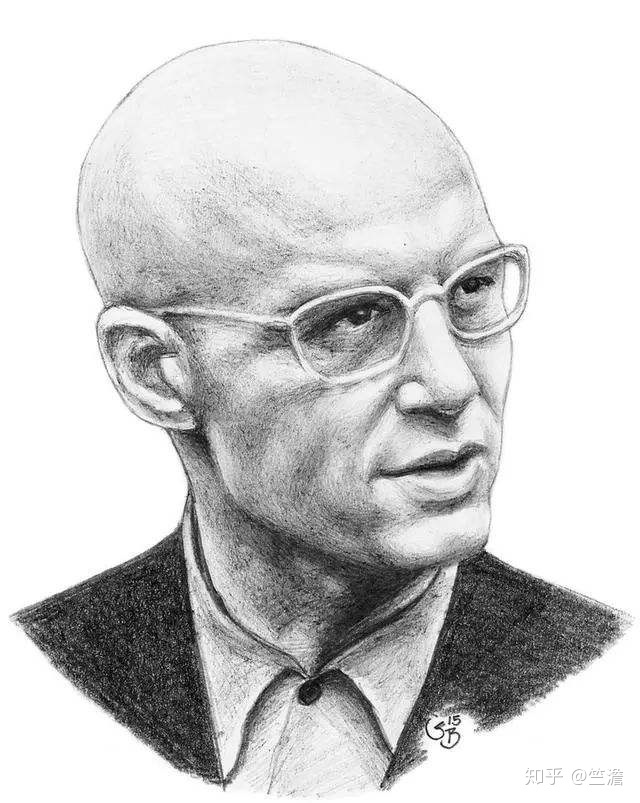
\includegraphics[width =3.4cm]{G1}}]
\begin{frame}[fragile]{Alexandre Grothendieck的贡献}
\begin{itemize}[<+-|alert@+>]
  \item 格罗滕迪克对代数几何进行了彻底的革命,建立新的基础,引入“概形”的概念,发表了十几本巨著,建立了一套宏大而完整的“概型理论”.格罗滕迪克的工作堪称代数几何的巅峰,他的著作被誉为“格罗滕迪克圣经”.格罗滕迪克的理论就发挥了价值.在概型理论的基础上,格罗滕迪克第一次给出了著名的黎曼-洛赫-格罗腾迪克定理的代数证明.
  \item 他在代数几何领域的成就大致可以分为10个方面:

(1) 连续与离散的对偶性 (寻来范畴,6种演算);

(2) Riemann-Roch-Grothendieck 定理  把 Riemann-Roch 定理由代数曲线和代数曲面推广到任意高维代数簇,其间发展了拓扑K理论;

(3) 概形 (Schemes) 概念的引入,使代数几何学还原为交换代数学;

(4) 拓扑斯 (Topos) 理论;

(5) 平展上同调与L进上同调;

(6) 动形 (motive) 理论;

(7) 晶状上同调 (Etale Cohomology);

(8) 拓扑斯 (Topos) 的上同调;

(9) 稳和拓扑;

(10) 非阿贝尔代数几何学.
\end{itemize}
\end{frame}

\begin{frame}
\frametitle{续接上面}
格罗滕迪克在代数几何领域取得了辉煌的成就,他的主要贡献在于他对代数几何发展的促进和影响. 他奠定了这门学科的理论基础, 并介绍了许多有用的数学工具. 代数几何通过代数方程研究几何对象,如代数曲线和曲面,利用环理论研究了代数方程的性质.

他还构造了上同调理论,并用代数技术研究拓扑对象,这在代数数论、代数拓扑和表示论中发挥了重要的作用和深远的影响.格罗滕迪克\alert{强调不同数学结构的共性,并将范畴理论纳入主流,成为数学的组织原则}. 他的阿贝尔范畴概念后来成为同调代数的基本框架和研究对象,他创立的拓扑理论是点集拓扑范畴理论的推广,它影响了集合论和数理逻辑.

他还构想了motif理论,推动了代数K理论、motif同伦论、motif积分的发展.他对几何学的贡献,也促进了数论的发展.他发现了上同调的第一个例子,开启了证明韦伊猜想的思路,启发了他的比利时学生皮埃尔•德利涅完成猜想的全部证明.值得提及的是,德利涅后来囊括了几乎全部最有名的数学大奖: 他1978年获菲尔兹奖、1988年获克拉福德奖、2008年获沃尔夫奖、2013年获阿贝尔奖.
\end{frame}

\section{Riemann-Roch-Grothendieck 定理}
\sepframe[title={Riemann-Roch-Grothendieck 定理}, image ={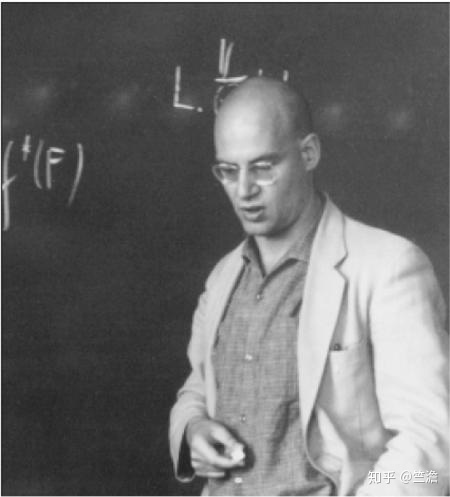
\includegraphics[width =3.4cm]{G2}}]
\begin{frame}
  \frametitle{An introduction to the Riemann-Roch-Hirzebruch Theorem}
  \pause[1]
\begin{lem}
  For all $j=0,1,\cdots$,  $\dim_{\mathbb{C}}H^j(M,\underline{E})<\infty$, and for all $j>\dim_{\mathbb{C}}(M)$, $H^j(M,\underline{E})=0$.
  We have 
  \[\chi (M,E):=\sum_{j=0}^{n}(-1)^j \dim_{\mathbb{C}}H^j(M,\underline{E}), \;\text{where}\; n=\dim_{\mathbb{C}}(M).\]
\end{lem}
\pause[2]
  \begin{thm}[][Hirzebruch-Riemann-Roch]
    Let $M$ be a non-singular projective algebraic variety $/\mathbb{C}$ and let $E$
be an algebraic vector bundle on $M$. Then
\[\chi (M,E)=(\mathrm{ch}(E)\cup \mathrm{Td}(M))[M].\]
  \end{thm}

\end{frame}

\section{Some remarks of the theorem}
\sepframe[title={Some remarks of the theorem}, image ={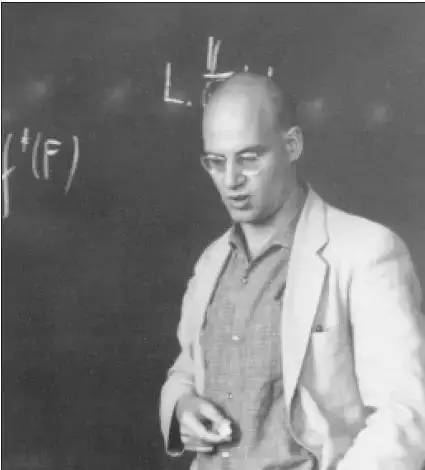
\includegraphics[width =3.4cm]{Grothendieck1}}]
\begin{frame}
  \frametitle{Some remarks of the theorem}
\pause[1]
  Idea : \textit{\textbf{The Hirzebruch-Riemann-Roch theorem}} identifies for a holomorphic vector bundle $E$ the alternating sum of its abelian sheaf cohomology groups (hence for trivial bundle the index of the Dolbeault operator) with the Chern character of the bundle cupped with the Todd class of the underlying complex manifold.

\pause[2]
\alert{Hirzebruch-Riemann-Roch定理}给出了全纯向量丛$E$的阿贝尔层上同调群 (因此对于平凡丛, Dolbeault算子的指标) 的交替和, 该丛具有Chern特征, 且与底部复流形的Todd类相依.
\end{frame}

\section{格罗滕迪克对该定理贡献}
\sepframe[title={格罗滕迪克对该定理贡献}, image ={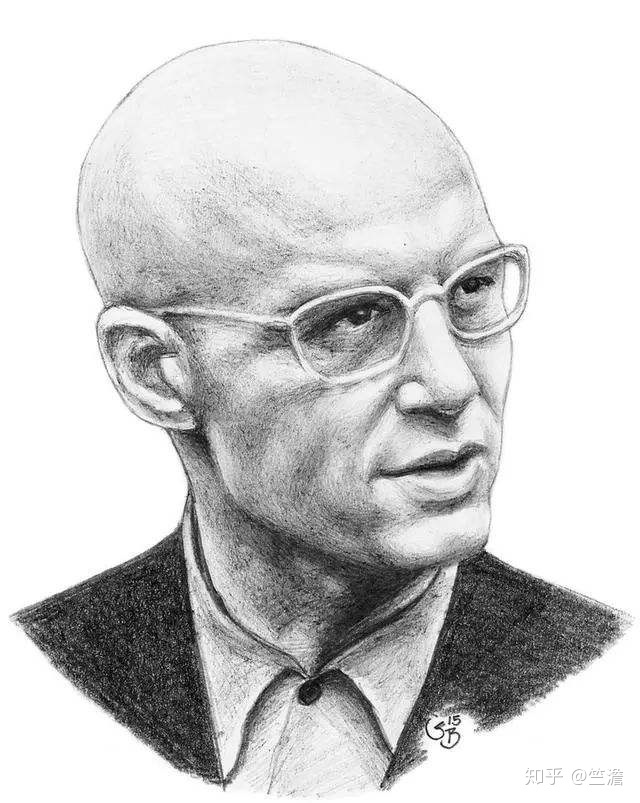
\includegraphics[width =3.4cm]{G1}}]
\begin{frame}
  \frametitle{格罗滕迪克对该定理贡献}
\pause[1]
  In 1957, A. Grothendieck generalized the Riemann-Roch-Hirzebruch theorem to the case of a morphism of non-singular varieties over an arbitrary algebraically closed field (see \cite{borel1958theoreme}). Let $K_0 X$ and $K^0 X$ be the Grothendieck groups of the coherent and locally free sheafs on $X$, respectively (\textit{Grothendieck group}). The functor $K_0 X$ is a covariant functor from the category of schemes and proper morphisms into the category of Abelian groups. In this case, for a proper morphism $f: X \rightarrow Y$ the morphism $f: K_0 X \rightarrow K_0 Y$ is defined by the formula
$$
f_{!}(\mathcal{F})=\sum(-1)^i R^i f_*(\mathcal{F})
$$
where $\mathcal{F}$ is an arbitrary coherent sheaf on $X$ and $K^0 X$ is a covariant functor into the category of rings. 

\pause[2]
For regular schemes with an ample sheaf, the groups $K_0 X$ and $K^0 X$ coincide and are denoted by $K(X)$. The Chern character ch : $K(X) \rightarrow H \cdot X$ is a homomorphism of rings; $H \cdot X$ is also a covariant functor: The Gizin homomorphism $f_*: H \cdot X \rightarrow H \cdot Y$ is defined. When $H \cdot X=H \cdot(X, \mathbf{Q})$, the homomorphism $f_*$ is obtained from $f_*$ for homology spaces using Poincaré duality. The theorem as generalized by Grothendieck expresses the measure of deviation from commutativity of the homomorphisms $f_{!}$and $\mathrm{ch}$.

\end{frame}


\begin{frame}
\pause[1]
  \begin{thm}[][Riemann-Roch-Hirzebruch-Grothendieck theorem]
    Let $f: X \rightarrow Y$ be a smooth projective morphism of non-singular projective varieties; then for any $x \in K(X)$ the equation
$$
\operatorname{ch}\left(f_{!}(x)\right)=f_*\left(\operatorname{ch}(x) \operatorname{td}\left(\mathcal{T}_f\right)\right)
$$
in $H \cdot X$ is true, where $\mathcal{T}_f=\mathcal{T}_X-f^*\left(\mathcal{T}_Y\right) \in K_X$ (the relative tangent sheaf of the morphism $f$ ).
  \end{thm}
  \pause[2]
When $Y$ is a point, this theorem reduces to the Riemann-Roch-Hirzebruch theorem. There are generalizations (see \cite{baum1979riemann,baum1975riemann,ferrand2006theorie}) when $Y$ is a Noetherian scheme with an ample invertible sheaf, when $f$ is a projective morphism whose fibres are locally complete intersections, and also to the case of singular quasi-projective varieties.

\end{frame}

\section{对格罗滕迪克的评价}
\begin{frame}[fragile]{对格罗滕迪克的评价}
\pause[1]
亚历山大-格洛腾迪克是一位对数学对象极度敏感, 对它们之间复杂而优美的结构有着深刻认识的数学家. 他生平中的两个制高点——他是高等科学研究所 (Institut des Hautes Études Scientifiques, IHÉS) 的创始成员之一, 并在 1966 年荣获菲尔兹奖——就足以保证他在二十世纪数学伟人殿里的位置. 但是这样的叙说远不足以反映他工作的精华,它深深植根于某种更有机更深层的东西里面. 正如他在长篇回忆录《收获与播种》中所说: \alert{“构成一个研究人员的创造力和想象力的品质的东西,正是他聆听事情内部声音能力”(原书第 27 页)}. 今天格洛腾迪克自己的声音,蕴含在他的著作中,到达我们耳中,就如来自虚空.  如今 76 岁的高龄,他已经在法国南部的一个小村落里隐居十多年了. 

\pause[2]
用密歇根大学 Hyman Bass 的话来说,格洛腾迪克\alert{用一种“宇宙般普适”的观点改变了整个数学的全貌}. 如今这种观点已经如此深入吸收到数学研究里面,以至于对新来的研究者来说,很难想象以前并不是这样的. \alert{格洛腾迪克留下最深印迹的是代数几何学,在其中他强调通过发现数学对象间的联系来理解数学对象本身. 他具有一种极其强大、几乎就是来自另外一个世界的抽象能力,让他能够从非常普适的高度来看待问题,而且他使用这种能力又是完美无缺的精确.} 事实上,从二十世纪中叶开始,在整个数学领域里不断加深的一般化和抽象化的潮流,在很大程度上归功于格洛腾迪克. 同时,那些为一般化而一般化,以至于去研究一些毫无意义或者没有意思的数学问题,是他从来不感兴趣的. 
\end{frame}

\begin{frame}[fragile]{续接上文}
  \begin{quotation}[-----------《收获与播种》,第 3 页]
      对于我来说,我们高中数学课本最令人不满意的地方,是缺乏对长度、面积和体积的严格定义. 我许诺自己,当我有机会的时候,我一定得填补这个不足. 
  \end{quotation}
  格罗腾迪克在泛函分析方面的工作“相当出色”,加州大学洛山矶分校的 Edwards E. Effors 评论说. “他可能是第一个意识到二战后迅猛发展的代数和范畴工具可以用来研究如此高度解析的数学分支泛函分析的人了. ”从某些方面来说,格洛腾迪克走在他的时代的前面,Effors 注意到至少花了 15 年时间,格洛腾迪克的工作才结合到主流的 Banach 空间理论中去,这其中部分原因是大家对采用他的更代数的观点不积极. Effors 还说道,近年来由于 Banach 空间理论的“量子化”,而格洛腾迪克的范畴论的方法特别适用于这种情况,他的工作的影响进一步得到加强. 
\end{frame}
  



\begin{frame}
  \frametitle{References}

  \printbibliography

\end{frame}


\thanksframe{谢谢大家的观看!}


\end{document} 